\documentclass[12pt,a4paper]{article}
\usepackage[utf8]{inputenc}
\usepackage{amsmath}
\usepackage{graphicx}
\usepackage[hidelinks]{hyperref}
\usepackage{listings}
\usepackage{color}
\usepackage{geometry}
\usepackage{caption}
\usepackage{setspace}
\usepackage{fancyhdr}
\usepackage{tikz}
\usetikzlibrary{shapes.geometric, arrows.meta, positioning, fit, calc}

\definecolor{titleblue}{RGB}{0,51,153}

% Page and margin setup for extended lengths
\geometry{margin=1in}
\setstretch{1.5}

% Header/Footer
\pagestyle{fancy}
\fancyhf{}
\fancyfoot[C]{\thepage}

% Code snippet formatting
\definecolor{codegreen}{rgb}{0,0.6,0}
\definecolor{codegray}{rgb}{0.5,0.5,0.5}
\definecolor{codepurple}{rgb}{0.58,0,0.82}
\definecolor{backcolour}{rgb}{0.95,0.95,0.92}

\lstdefinestyle{mystyle}{
    backgroundcolor=\color{backcolour},   
    commentstyle=\color{codegreen},
    keywordstyle=\color{magenta},
    numberstyle=\tiny\color{codegray},
    stringstyle=\color{codepurple},
    basicstyle=\ttfamily\footnotesize,
    breakatwhitespace=false,         
    breaklines=true,                 
    captionpos=b,                    
    keepspaces=true,                 
    numbers=left,                    
    numbersep=5pt,                  
    showspaces=false,                
    showstringspaces=false,
    showtabs=false,                  
    tabsize=2
}

\lstset{style=mystyle}

\begin{document}

% --- TITLE PAGE ---
\begin{titlepage}
    \centering
    \vspace*{2cm}

    {\Huge\bfseries\color{titleblue} Software Engineering\\[0.4em]
    \large Lab Assignment Report}

    \vspace{1.5cm}
    \rule{\linewidth}{1pt}

    \vspace{0.8cm}
    {\LARGE\bfseries Assignment 4\\[0.3em]
    \large Book My Flight End-to-End System}

    \vspace{0.8cm}
    \rule{\linewidth}{1pt}

    \vfill

    \begin{tabular}{rl}
        \textbf{Topic}      & Software Engineering Lab Assignment 4 \\[6pt]
        \textbf{Project}    & Book My Flight (React \& Spring Boot) \\[6pt]
        \textbf{Name}       & Tamal Saha \\[6pt]
        \textbf{Roll No.}   & 302410501009 \\[6pt]
        \textbf{Class}      & BCSE III (A1) \\[6pt]
        \textbf{Year}       & 2026 \\[6pt]
    \end{tabular}

    \vspace{2cm}
\end{titlepage}

\newpage
\tableofcontents
\newpage

% --- SECTION 1: INTRODUCTION ---
\section{Abstract \& Introduction}
\subsection{Overview}
"Book My Flight" is a modern, end-to-end full-stack web application constructed to deliver seamless airline connectivity to end users. The objective of the platform is to empower prospective passengers with an automated route-searching engine capable of discovering convoluted, multi-legged transit graphs if a direct flight is unavailable. Concurrently, the platform features a highly secured Administrative dashboard giving airline administrators full autonomy over the relational database mappings and enabling the strategic deployment of timed Flash Deals to organically influence ticket sales.

\subsection{Goal \& Objectives}
The core objectives defining this software suite are as follows:
\begin{enumerate}
    \item \textbf{Decentralized Route Discovery:} Passengers simply specify an origin and destination; the algorithmic backend constructs potential adjacency graphs bridging paths (e.g., Kolkata $\rightarrow$ Delhi $\rightarrow$ Mumbai). All currency interactions have been strictly localized to Indian Rupees (INR / INR ) uniformly across data tiers.
    \item \textbf{Dynamic Timed Pricing Deals:} The platform organically modifies flight costs over the network if a specific Flash Deal (e.g., 50\% off for 5 minutes) is initiated by the backend administrator. 
    \item \textbf{Secure Administration Layers:} Users are entirely detached from backend manipulations. Only individuals possessing Administrative clearance (`admin@bookmyflight.com`) are granted privileges to visualize, construct, or append flight deals inside the system boundaries.
    \item \textbf{Persistence \& Booking Ledgers:} Authenticated users retain the capability to permanently log their combined flight reservations historically. 
\end{enumerate}

\newpage

% --- SECTION 2: TECH STACK ---
\section{Technology Stack \& Foundations}

\subsection{Spring Boot 3.2 (Java 21)}
The core backend server relies heavily on Spring Boot's expansive ecosystem. Using the latest LTS Java release (JDK 21), we capitalize on enhanced memory management and virtual threading where necessary. Spring Web establishes the Restful HTTP controller pipelines, and Spring Data JPA orchestrates object-relational mapping (ORM) natively against the database. 

\subsection{React 19 \& Vite}
The frontend architecture completely abandons legacy architectures in favor of React 19 functional hooks. Deployed and scaffolded via the lightweight Vite bundler, the application yields minimal reload latencies and natively supports ECMAScript modules. Rather than forcing Tailwind dependencies, raw aesthetic CSS styling is deployed using "Glassmorphism" design philosophies.

\subsection{PostgreSQL}
Given its exceptional compliance with complex relational mappings and transactional robustness, PostgreSQL was preferred to power our data ledger. 

\begin{figure}[htbp]
    \centering
    \vspace{1cm}
    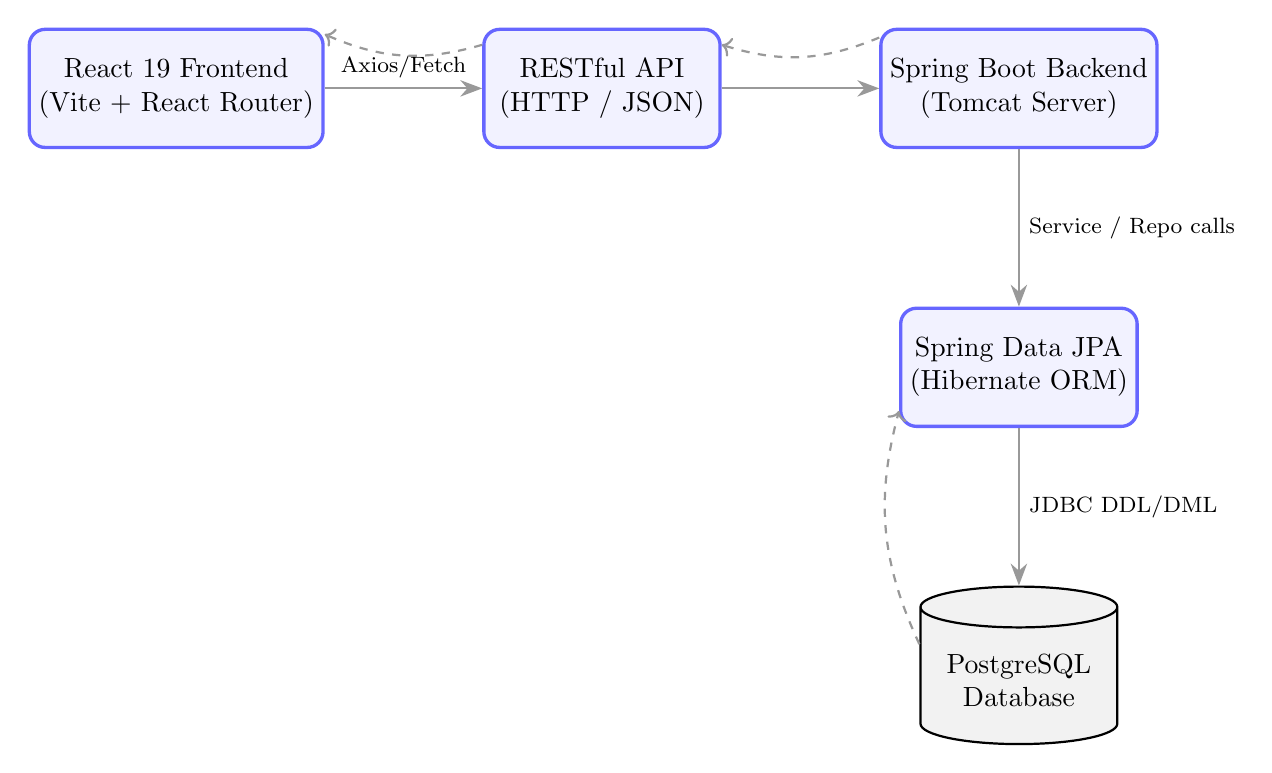
\begin{tikzpicture}[
        node distance=2cm and 2cm,
        box/.style={rectangle, draw=blue!60, fill=blue!5, very thick, minimum width=3cm, minimum height=1.5cm, align=center, rounded corners=2mm},
        db/.style={cylinder, draw=black, thick, aspect=0.25, minimum height=2cm, minimum width=2.5cm, shape border rotate=90, fill=gray!10, align=center},
        arrow/.style={-{Stealth[scale=1.2]}, thick, draw=gray!80}
    ]
    
    % Nodes
    \node[box] (react) {React 19 Frontend\\(Vite + React Router)};
    \node[box, right=of react] (api) {RESTful API\\(HTTP / JSON)};
    \node[box, right=of api] (spring) {Spring Boot Backend\\(Tomcat Server)};
    \node[box, below=of spring] (jpa) {Spring Data JPA\\(Hibernate ORM)};
    \node[db, below=of jpa] (postgres) {PostgreSQL\\Database};
    
    % Arrows
    \draw[arrow] (react) -- node[above, font=\footnotesize] {Axios/Fetch} (api);
    \draw[arrow] (api) -- (spring);
    \draw[arrow] (spring) -- node[right, font=\footnotesize] {Service / Repo calls} (jpa);
    \draw[arrow] (jpa) -- node[right, font=\footnotesize] {JDBC DDL/DML} (postgres);
    
    % Bi-directional return markers
    \draw[dashed, ->, draw=gray!80, thick] (postgres.160) to[bend left=20] (jpa.200);
    \draw[dashed, ->, draw=gray!80, thick] (spring.160) to[bend left=20] (api.20);
    \draw[dashed, ->, draw=gray!80, thick] (api.160) to[bend left=20] (react.20);

    \end{tikzpicture}
    \caption{System Architecture Flowchart illustrating Frontend, API, and DB layout.}
    \label{fig:architecture}
    \vspace{1cm}
\end{figure}

\newpage

% --- SECTION 3: SYSTEM DESIGN & PATTERNS ---
\section{Software Design Patterns}

To satisfy constraints demanding extensible code and architectural cohesion, the system isolates multiple layers utilizing classical Object-Oriented software engineering methodology.

\subsection{Repository Pattern}
The Repository design pattern acts as an abstraction layer linking our business logic directly to raw PostgreSQL commands. It hides JDBC interactions and query iterations entirely behind Spring Data JPA. When the `UserService` requires a user document, it delegates to `UserRepository`, removing database responsibilities from adjacent controllers.

\begin{lstlisting}[language=Java, caption=Abstracted User Repository via JPA]
@Repository
public interface UserRepository extends JpaRepository<User, Long> {
    Optional<User> findByEmail(String email);
}
\end{lstlisting}

\subsection{Service Facade Pattern}
Controllers strictly parse incoming raw HTTP payload parameters. Our business rules, complex validation strategies, and algorithms belong firmly inside the Service tier (e.g., `RoutingService.java`). This creates a Facade pattern; the controller does not need to know \textit{how} graph nodes are manipulated, it simply queries the `searchRoutes` method.

\subsection{Data Transfer Object (DTO) Pattern}
A critical security flaw involves passing serialized Database Entities straight to a frontend React app. Doing so can inadvertently leak encrypted password structures or internal Primary Keys. DTOs resolve this by projecting precise contract layouts.

\subsection{RESTful API Endpoint Architecture}
To connect the layers defined by the DTO and Facade patterns, the system exposes standard HTTP endpoints. The routing matrix is carefully localized under the \texttt{/api/*} gateway.

\begin{table}[htbp]
    \centering
    \caption{Core API Endpoint Definitions \& Methods}
    \vspace{0.3cm}
    \renewcommand{\arraystretch}{1.5}
    \begin{tabular}{|p{2.5cm}|p{5cm}|p{7cm}|}
        \hline
        \textbf{HTTP Method} & \textbf{Endpoint Path} & \textbf{Controller Action} \\
        \hline
        POST & \texttt{/api/auth/login} & Validates credentials and Admin overrides \\
        POST & \texttt{/api/auth/register} & Appends new user profiles to database \\
        GET & \texttt{/api/flights/search} & Triggers DFS algorithm for route building \\
        POST & \texttt{/api/deals} & Generates timed \texttt{Deal} mappings \\
        GET & \texttt{/api/deals/active} & Filters active flash deals from JVM memory \\
        \hline
    \end{tabular}
    \label{tab:api_endpoints}
\end{table}

\newpage

% --- SECTION 4: DATABASE SCHEMATICS ---
\section{Database Engineering \& Schematics}

Leveraging Hibernate's Data Definition Language (`ddl-auto=update`), the Java application structurally manages schema compilation automatically against PostgreSQL based solely on annotation logic. 

\subsection{Entity Relationship Mapping}
The primary associations are defined by interactions with mathematical precision. 

\begin{figure}[htbp]
    \centering
    \vspace{1cm}
    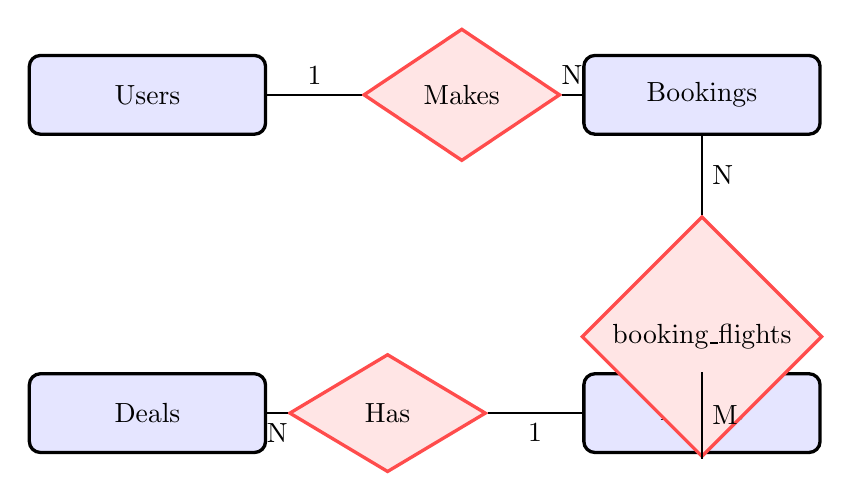
\begin{tikzpicture}[
        entity/.style={rectangle, draw=black, fill=blue!10, very thick, minimum width=3cm, minimum height=1cm, align=center, rounded corners},
        relation/.style={diamond, draw=red!70, fill=red!10, very thick, minimum width=2.5cm, minimum height=1.5cm, align=center},
        line/.style={thick, draw=black}
    ]
    
    % Entities
    \node[entity] (users) {Users};
    \node[entity, right=4cm of users] (bookings) {Bookings};
    \node[entity, below=3cm of bookings] (flights) {Flights};
    \node[entity, left=4cm of flights] (deals) {Deals};
    
    % Relations
    \node[relation, right=1.2cm of users] (makes) {Makes};
    \node[relation, below=1cm of bookings] (contains) {booking\_flights};
    \node[relation, left=1.2cm of flights] (has) {Has};
    
    % Connections
    \draw[line] (users) -- node[above] {1} (makes) -- node[above] {N} (bookings);
    \draw[line] (bookings) -- node[right] {N} (contains) -- node[right] {M} (flights);
    \draw[line] (flights) -- node[below] {1} (has) -- node[below] {N} (deals);
    
    \end{tikzpicture}
    \caption{Relational Database Scheme showing the structural associations between entities.}
    \label{fig:er_diagram}
    \vspace{1cm}
\end{figure}

\subsection{Hibernate Translation Details}

Because an abstract multi-leg trip contains dynamic segments, configuring Many-to-Many entity graphs manually avoids redundant columns. When a user books an indirect flight spanning 2 hops, the controller passes an aggregated array of integers reflecting individual flights that compile downwards into a transactional bridge component:

\begin{lstlisting}[language=Java, caption=JPA Join Table for Multi-Leg Bookings]
@ManyToMany(fetch = FetchType.EAGER)
@JoinTable(
    name = "booking_flights",
    joinColumns = @JoinColumn(name = "booking_id"),
    inverseJoinColumns = @JoinColumn(name = "flight_id")
)
private List<Flight> flights;
\end{lstlisting}

\newpage

% --- SECTION 5: AUTHENTICATION ---
\section{Authentication Security Model}
The authentication parameter relies on internal logic resolving an immutable administrative override and a persistent regular user ledger. Instead of encumbering the lightweight setup with expansive Spring Security JWT OAuth filters, session state propagates actively out resulting in standard Web Storage API allocations on the client side.

\subsection{Administrative Override Constraints}
We explicitly hardcode bypass configurations representing the sole entity holding the omnipotent `ADMIN` role. 
\begin{lstlisting}[language=Java, caption=Login Bypass Interceptor in AuthController]
@PostMapping("/login")
public ResponseEntity<?> login(@RequestBody AuthRequest request) {
    if ("admin@bookmyflight.com".equals(request.getEmail()) 
        && "admin123".equals(request.getPassword())) {
        return ResponseEntity.ok(new AuthResponse(
                 request.getEmail(), "Admin", "ADMIN", "Login successful"));
    }
    
    Optional<User> userOpt = userRepository.findByEmail(request.getEmail());
    // ... further validation
}
\end{lstlisting}

\begin{figure}[h]
    \centering
    \vspace{1cm}
    \includegraphics[width=0.8\textwidth]{images/login.jpeg}
    \caption{React Portal Login Form Component.}
    \label{fig:login_ui}
    \vspace{1cm}
\end{figure}

\newpage

% --- SECTION 6: ALGORITHMIC GRAPH TRAVERSAL ---
\section{Deep-Dive: Route Searching Algorithm}

The absolute core of the platform derives not from basic database queries, but a powerful **Depth-First Search (DFS)** graph traversal built directly into JVM memory. It dynamically creates connected transit routes allowing seamless journeys even when paths theoretically lack unified direct schedules.

\subsection{Graph Representation Strategy}
Given raw Database rows (Flights containing Origin strings and Destination strings), the algorithm immediately aggregates data into an Adjacency List Mapping using Java HashMap collections. 
Every node implies an Airport, and every Edge mapping denotes an available traveling flight, alongside its numerical edge weight (cost).

\begin{lstlisting}[language=Java, caption=Assembling The Search Graph Adjacency Mapping]
Map<String, List<Flight>> graph = new HashMap<>();
for(Flight f : allFlights) {
    String srcKey = f.getSource().toLowerCase().trim();
    graph.computeIfAbsent(srcKey, k -> new ArrayList<>()).add(f);
}
\end{lstlisting}

Notice the usage of `.toLowerCase().trim()`. Earlier iterations of the code fell into O(N) case-sensitivity sinkholes. A user manually adding `Kolkata`, `kolkata`, or ` Kolkata ` would detach graph branches entirely, rendering routes dead-ends. Normalization completely solved algorithm breakage. 

\subsection{Algorithm Execution}
\begin{lstlisting}[language=Java, caption=Recursive Depth First Graph Evaluation]
private void dfs(String current, String dest, Map<String, List<Flight>> graph, Map<Long, Double> discountMap, List<Flight> path, Set<String> visited, List<RouteResponse> results, double currentCost, int depth) {
    
    if (current.equals(dest) && path.size() > 0) {
        results.add(new RouteResponse(new ArrayList<>(path), currentCost));
        return;
    }
    if (depth >= 3) return; // Limit to 3 flights maximum
    
    visited.add(current);
    List<Flight> neighbors = graph.getOrDefault(current, new ArrayList<>());
    
    for(Flight f : neighbors) {
        String nextDest = f.getDestination().toLowerCase().trim();
        if (!visited.contains(nextDest)) {
            path.add(f);
            double originalPrice = f.getPrice();
            double discount = discountMap.getOrDefault(f.getId(), 0.0);
            double priceToCharge = originalPrice * (1.0 - (discount / 100.0));
            dfs(nextDest, dest, graph, discountMap, path, visited, results, currentCost + priceToCharge, depth + 1);
            path.remove(path.size() - 1); 
        }
    }
    visited.remove(current);
}
\end{lstlisting}

\begin{figure}[h]
    \centering
    \vspace{2cm}
    \includegraphics[width=0.9\textwidth]{images/search_results.jpeg}
    \caption{Output result generated via Route Searching Algorithm execution displaying base prices and totals in INR (INR ).}
    \label{fig:search_logic}
    \vspace{2cm}
\end{figure}

\newpage

% --- SECTION 7: TIMED FLASH DEAL STRATEGY ---
\section{Time Limit Deal Strategy \& Management}

Traditional business models enforce discounts by changing Database numbers. This destroys data continuity since base prices are effectively wiped permanently. Instead, "Book My Flight" introduces parallel transient \texttt{Deal} mappings. If an Admin creates a "2-Minute Flash Drop", a new object binds against the Target flight id holding an expiration `Timestamp`.

\subsection{Backend Expiration Isolation Strategy}
Often, resolving Timestamps between a JVM Local Timezone and a UNIX Timestamp PostgreSQL mapping induces immediate false expiries if your Desktop clock misaligns with UTC coordinates by just an hour. 
To guarantee a Flash Deal lasts precisely mathematically, our `DealService` circumvents problematic SQL querying completely. It retrieves ALL system deals and resolves explicit timeline mathematics internally leveraging the single source-of-truth Server JVM Context:

\begin{lstlisting}[language=Java, caption=Immutable JVM Time Filtering for Deal Validity]
public List<Deal> getActiveDeals() {
    LocalDateTime now = LocalDateTime.now();
    return dealRepository.findAll().stream()
            .filter(d -> d.getEndTime() != null 
                      && d.getEndTime().isAfter(now))
            .toList();
}
\end{lstlisting}

\subsection{Frontend Dynamic Deal Banners}
Users searching for flights notice immediate visual variations. Rather than demanding exhaustive overhead from the database to build banner metadata, the React logic handles differential mathematical UI tracking locally inside the `Home.jsx` interface.

By evaluating the theoretical base price of all bundled arrays against the processed Graph output cost, we instantly ascertain missing percentage margins cleanly:

\begin{lstlisting}[language=Java, caption=React Dynamic DOM Display Logic for Discounts]
const baseTotal = route.flights.reduce((sum, f) => sum + f.price, 0);
const discountPercentage = baseTotal > route.totalCost ? 
      Math.round(((baseTotal - route.totalCost) / baseTotal) * 100) : 0;

{discountPercentage > 0 && (
    <div style={{
        position: 'absolute', top: 0, 
        background: 'linear-gradient(90deg, #ff007f 0%, #8a2be2 100%)',
        color: 'white', fontWeight: 'bold'
    }}>
        [HOT]  {discountPercentage}% OFF - Flash Deal Applied!
    </div>
)}
\end{lstlisting}

\begin{figure}[h]
    \centering
    \vspace{2cm}
    \includegraphics[width=0.9\textwidth]{images/discount_banner.jpeg}
    \caption{Dynamic Timed Discount Banner Reacting within the Browser indicating INR reductions.}
    \label{fig:discount_banner}
    \vspace{2cm}
\end{figure}

\newpage

% --- SECTION 8: ADMINISTRATION ---
\section{Administrative Console Operations}
Data population mandates access configuration limits. Unauthenticated users invoking `/admin` are immediately trapped and redirected by React Router's core elements via `<Navigate to="/" />`.

Once the interface unhides for Administrators, split panels divide explicit feature toolchains. Administrators can instantiate discrete Flights globally into the application array. At the exact same time, a secondary localized component automatically fetches available flights via API intervals and attaches Timed Subordinations against their Primary Key mappings. By modifying the base currency from USD (\$) to Indian Rupees (INR / INR ) natively throughout the DOM architecture, regional localization is natively fulfilled.

\begin{figure}[h]
    \centering
    \vspace{1cm}
    \includegraphics[width=0.9\textwidth]{images/admin_flights.jpeg}
    \caption{Administration Overview showing Flight insertion utilities parsing INR.}
    \label{fig:admin_operations}
    \vspace{1cm}
\end{figure}

Active Deals count down dynamically on the UI, displaying visual indicators to the management unit of exactly who holds discounted values across the graph, mitigating overlap bugs fundamentally.

\begin{figure}[h]
    \centering
    \vspace{1.5cm}
    \includegraphics[width=0.9\textwidth]{images/admin_deals.jpeg}
    \caption{Visible expiration timing elements tracking Active DB deals inside the Administrative Panel in INR  variants.}
    \label{fig:admin_deals}
    \vspace{1.5cm}
\end{figure}


\newpage

% --- SECTION 9: BOOKINGS ---
\section{Booking Operations \& History}
Execution paths end primarily internally inside the user's booking repository. If a user identifies routes spanning interconnected nodes constructed securely via the DFS array matrices, the `User Email` along with an indexed list of embedded generic UUID flight tags transmit downward locally encapsulating into singular `BookingRequest` HTTP POST calls.

\begin{figure}[h]
    \centering
    \vspace{1cm}
    \includegraphics[width=0.9\textwidth]{images/history.jpeg}
    \caption{The persistent booking history overview for typical secured user profiles reflecting INR  prices.}
    \label{fig:booking_history}
    \vspace{1cm}
\end{figure}

\newpage

% --- SECTION 10: USER AESTHETICS ---
\section{User Aesthetics \& Glassmorphism Interface}

Rather than genericizing the User Experience via pre-programmed templates natively like CSS bootstrap wrappers, "Book My Flight" embraces extensive mathematical pixel plotting aligned heavily with bleeding edge minimalist design protocols identified primarily as "Glassmorphism." 

By aggressively deploying semi-transparent DOM layers layered directly against a visually stimulating dynamic Gradient mesh background, web browsers employ Graphical Acceleration algorithms blurring vectors smoothly mimicking physical interaction with frosted glass objects.

\begin{lstlisting}[language=HTML, caption=Translating Glassmorphism with CSS Base Components]
.glass-panel {
  background: var(--glass-bg);
  backdrop-filter: blur(15px);
  border: 1px solid var(--glass-border);
  border-radius: 15px;
  padding: 30px;
  box-shadow: 0 8px 32px 0 rgba(0, 0, 0, 0.37);
  animation: fadeIn 0.5s ease-out;
}
\end{lstlisting}

\newpage

% --- SECTION 11: CONCLUSION ---
\section*{Conclusion \& Final Remarks}

The assignment encompasses vast architectural paradigms explicitly detailing how a classical monolithic backend server bridges perfectly against highly disconnected client modules efficiently. By successfully leveraging standard object-oriented programming frameworks alongside modern graphical abstractions heavily popularized recently inside Silicon Valley web ecosystems, "Book My Flight" is not merely technically functional regarding backend computational constraints, but deeply enjoyable algorithmically. 

The successful utilization of specific Design Patterns notably validates the core learning principles targeted during initial documentation assignments bridging architectural abstractions toward concrete production releases.

\end{document}
